\documentclass[11pt,UTF8]{ctexart}
\title{单个圆形固体颗粒悬浮于库埃特流}
\author{马坤}
\date{2019.11.5}
\usepackage{amsmath}
\usepackage{graphicx}
\usepackage{caption}
\usepackage{subcaption}
\usepackage[left=1in, right=1in, top=1in, bottom=1in]{geometry}
\begin{document}
    \maketitle
    在这个情况下,上固体板以速度为$U_0=0.1$移动,圆形固体
    颗粒的圆心处于库埃特流体模拟区域的中央;其半径为$r=H/4$
    ,$H=1$是模拟区域的宽度,模拟区域的长度为$L=H=1$;流体与
    颗粒的密度都假设为$\rho=1$;此次模拟中我们假设$W=0.1$。
    我们的$\phi$形式如下:
    $$
    \phi=0.5[-\tanh{\frac{2.4(r-1/4)}{W}}+1], r=\sqrt{(x-L/2)^2+(y-H/2)^2}.\eqno(1)
    $$
    \par{$\phi$应该是一个二元函数,图1.a为其三维图片,图1.b为$\phi$在$x=0.5$或者$y=0.5$
    处的投影。在给出的数值的情况下,$\phi$在固体颗粒里面$(r < H/4)$
    为1,在固体外面的液体里面$(r > H/4)$为0,固液交界面$(r = H/4)$为0.5。}
    \begin{figure}[b]
        \centering
        \begin{subfigure}[t]{0.49\textwidth}
            \centering
            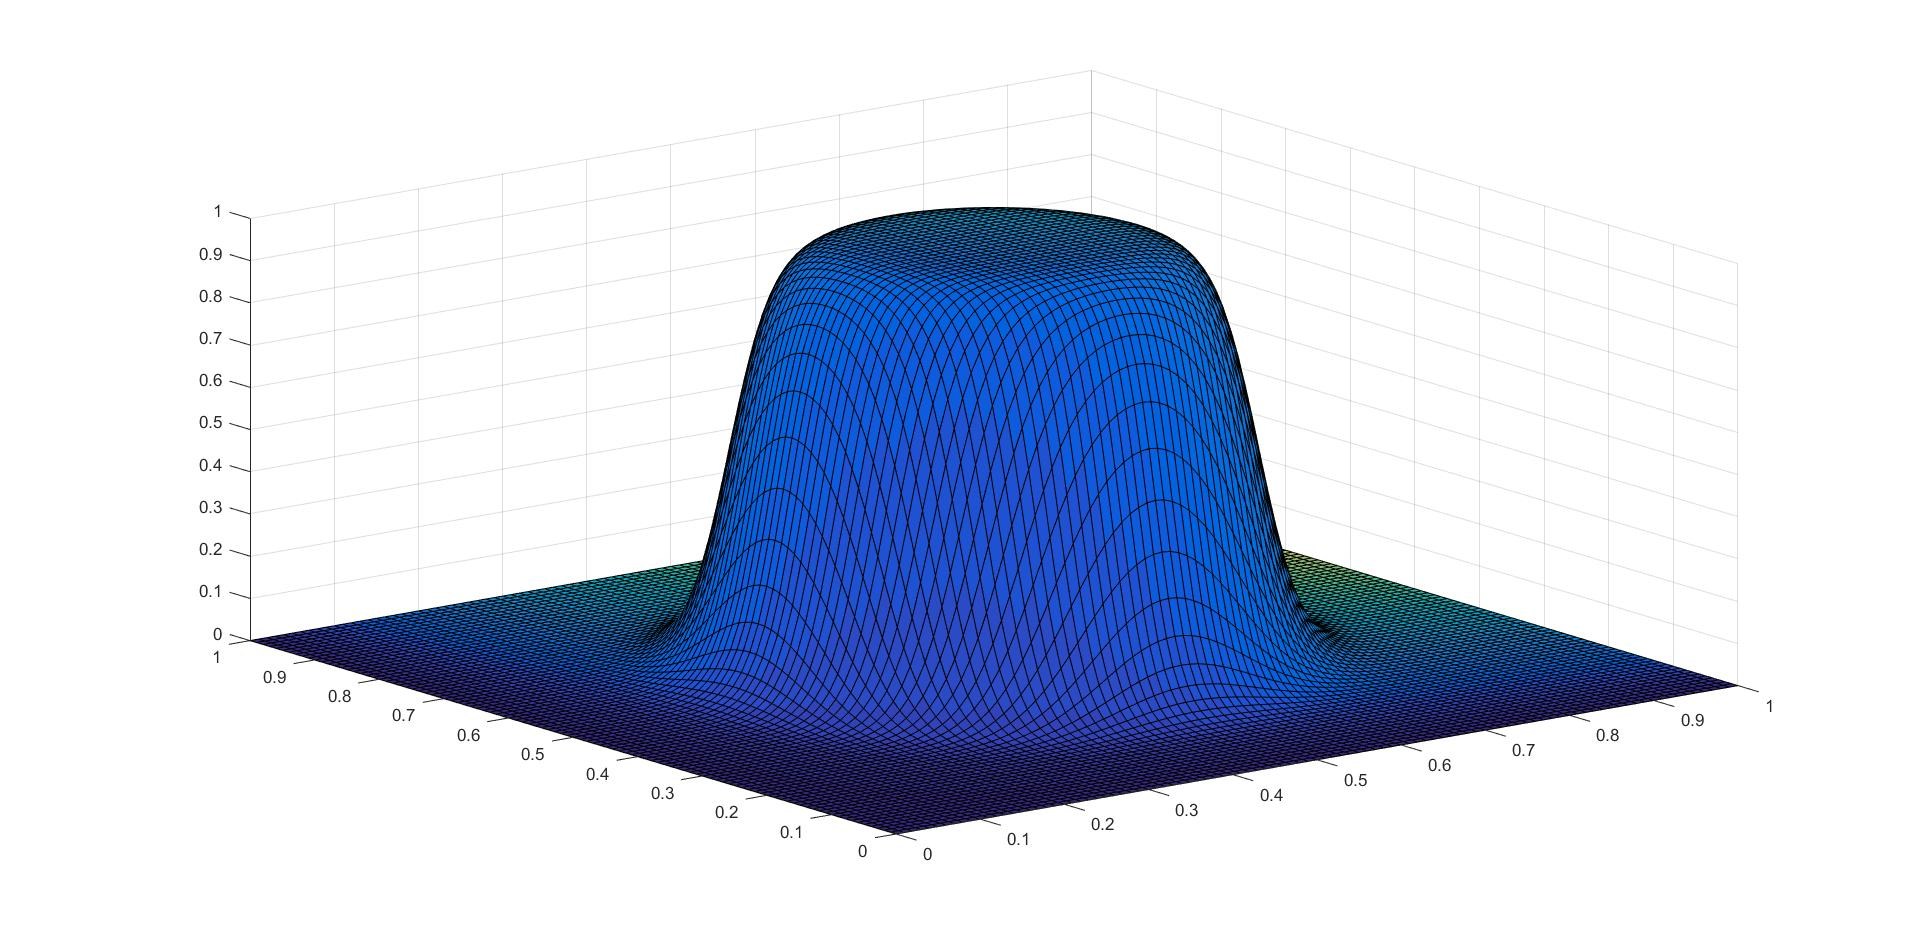
\includegraphics[width=\textwidth]{3D.jpg}
            \caption{$\phi$的3维图片}\label{1.a}
        \end{subfigure}
        \begin{subfigure}[t]{0.49\textwidth}
            \centering
            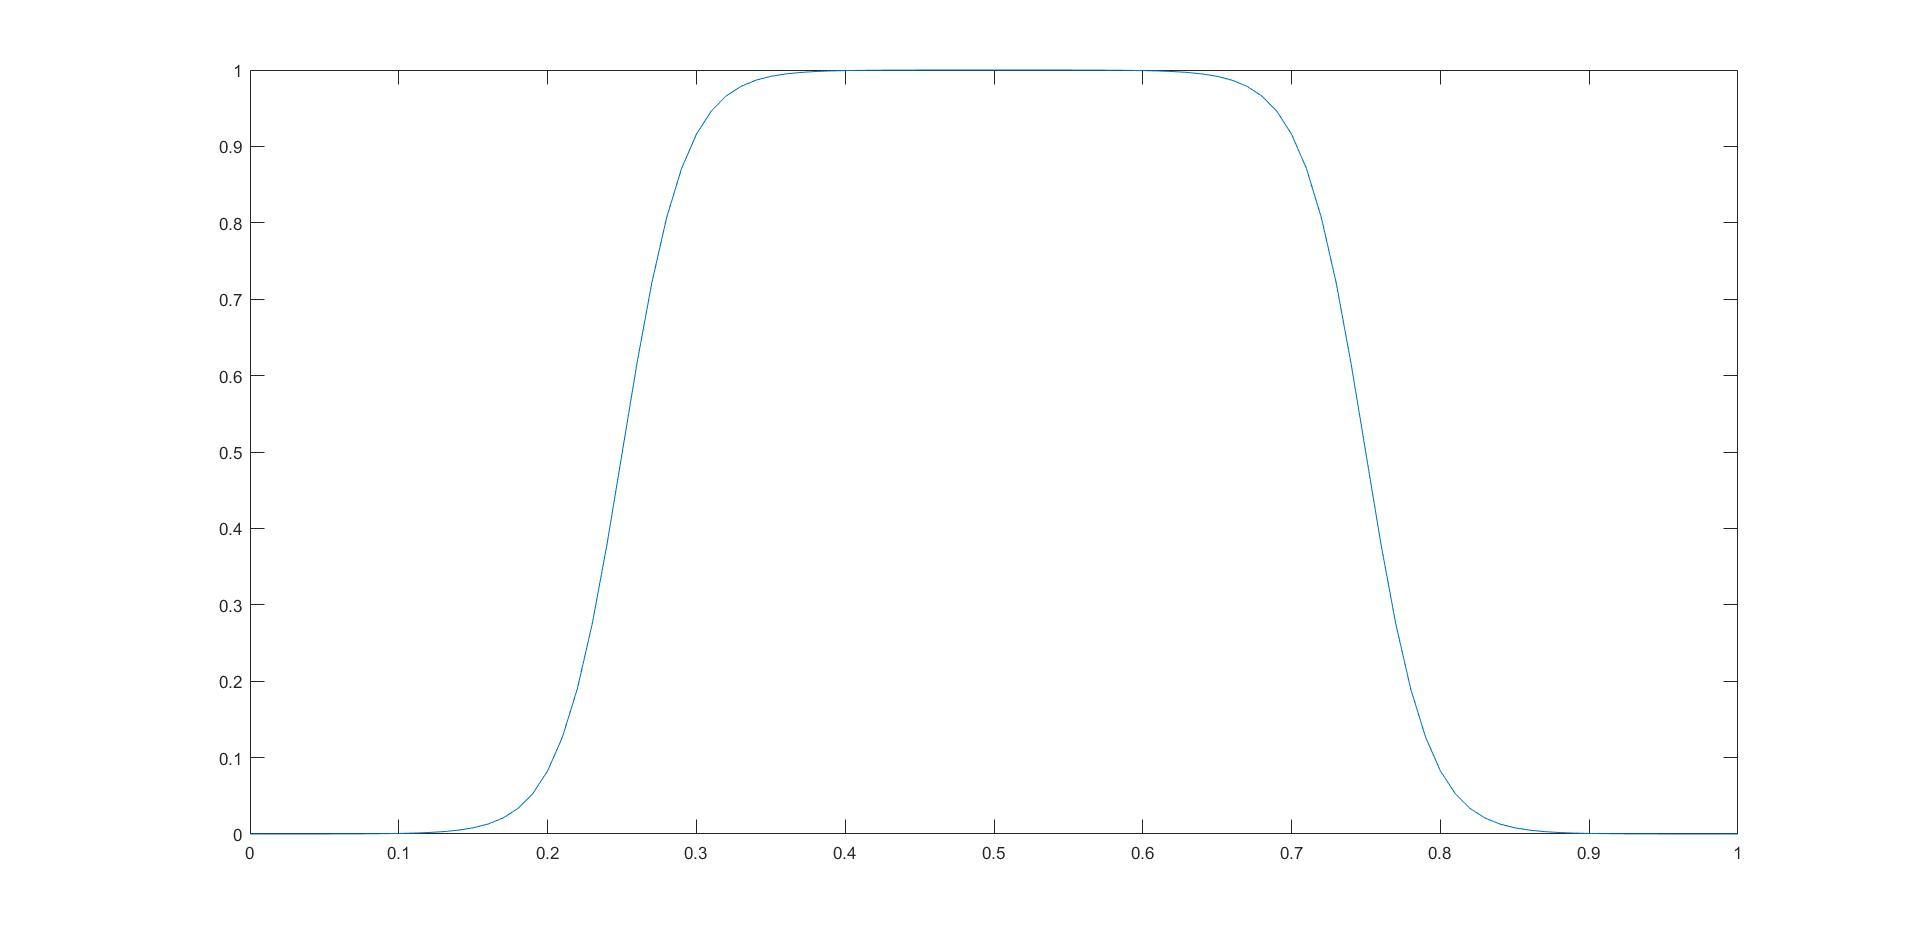
\includegraphics[width=\textwidth]{untitled.jpg}
            \caption{$\phi$在$x=0.5$$(y=0.5)$的投影}\label{1.b}
        \end{subfigure}
        \caption{$\phi$的图像}
    \end{figure}
    \par{模拟中我们假设$\frac{\eta_s}{\eta_l}=50$,我们的粘
    性系数$\eta$有如下表达式:
    $$\eta = 1+\frac{\eta_s}{\eta_l}\phi-\phi.\eqno(2)$$
    可以知道我们的$\eta$的极大值为50,为了和黄老师的论文进行匹配,在数值模拟中
    雷诺数$Re=500$。}
    \par{由于假设的流体与颗粒的密度都假设为$\rho=1$,所以有$\eta
    =\nu$,这会在数值模拟中用到。库埃特流的控制方程与解可以写为:}
    $$\nabla p=\nabla\cdot(\eta\nabla u).\eqno(3)$$
    $$u_x=U_0\frac{y}{H},u_y=0.\eqno(4)$$
    本来原始的库埃特流控制方程中$\nabla p=0$,但是此处粘性系数是关于
    位置的函数,所以压强的梯度一定不为0。于是方程就和泊肃叶流的控制方程
    一致,化简控制方程$(3)$得到:
    $$\nabla p=(\nabla u)\nabla \eta  + \eta \triangle u.\eqno(5)$$
    其中
    $$
    \nabla u=\left(
    \begin{array}{cc}
        0 & U_0/H \\
        0 & 0
    \end{array}
    \right).\eqno(6)
    $$
    $$\triangle u=\left(
    \begin{aligned}
    0 \\
    0
    \end{aligned}
    \right).\eqno(7)
    $$
    $$\nabla \eta=(\frac{\eta_s}{\eta_l}-1)\nabla \phi.\eqno(8)$$
    我们可以利用$\phi,\eta$定义表达式$(1),(2)$计算得到:
    $$\nabla \eta=
        (\frac{\eta_s}{\eta_l}-1)\{-0.5[1-\tanh^2\frac{2.4(r-1/4)}{W}]\frac{2.4}{W}\nabla r\}
    $$
    $$
    where\nabla r=\left(
        \begin{aligned}
            \frac{x-L/2}{\sqrt{(x-L/2)^2+(y-H/2)^2}}    \\
            \frac{y-H/2}{\sqrt{(x-L/2)^2+(y-H/2)^2}}
        \end{aligned}
    \right).\eqno(9)
    $$
    \par{将$(6)(7)(8)(9)$代入$(5)$,得到:
    $$
        \nabla p =\left(
            \begin{array}{cc}
                U_0(\frac{\eta_s}{\eta_l}-1)
                \{-0.5[1-\tanh^2\frac{2.4(r-1/4)}{W}]\frac{2.4}{W}\frac{y-H/2}{\sqrt{(x-L/2)^2+(y-H/2)^2}}\}/H \\
                0
            \end{array}
            \right).\eqno(10)
    $$
    }
    \par{由于外力与压强有如下关系$F = -\nabla p$,再代入所有实验数值,
    我们可以得到外力的精确表达式,由于压强的$y$方向梯度为0,在$y$方向没有
    力,下面表达式只写$x$方向的力。
    $$
        F =58.8(y-1/2)
        [1-\tanh^2 {24(r-1/4)}]/r.\eqno(11)
    $$
    
    \begin{figure}[t]
        \centering
        \begin{subfigure}[t]{0.49\textwidth}
            \centering
            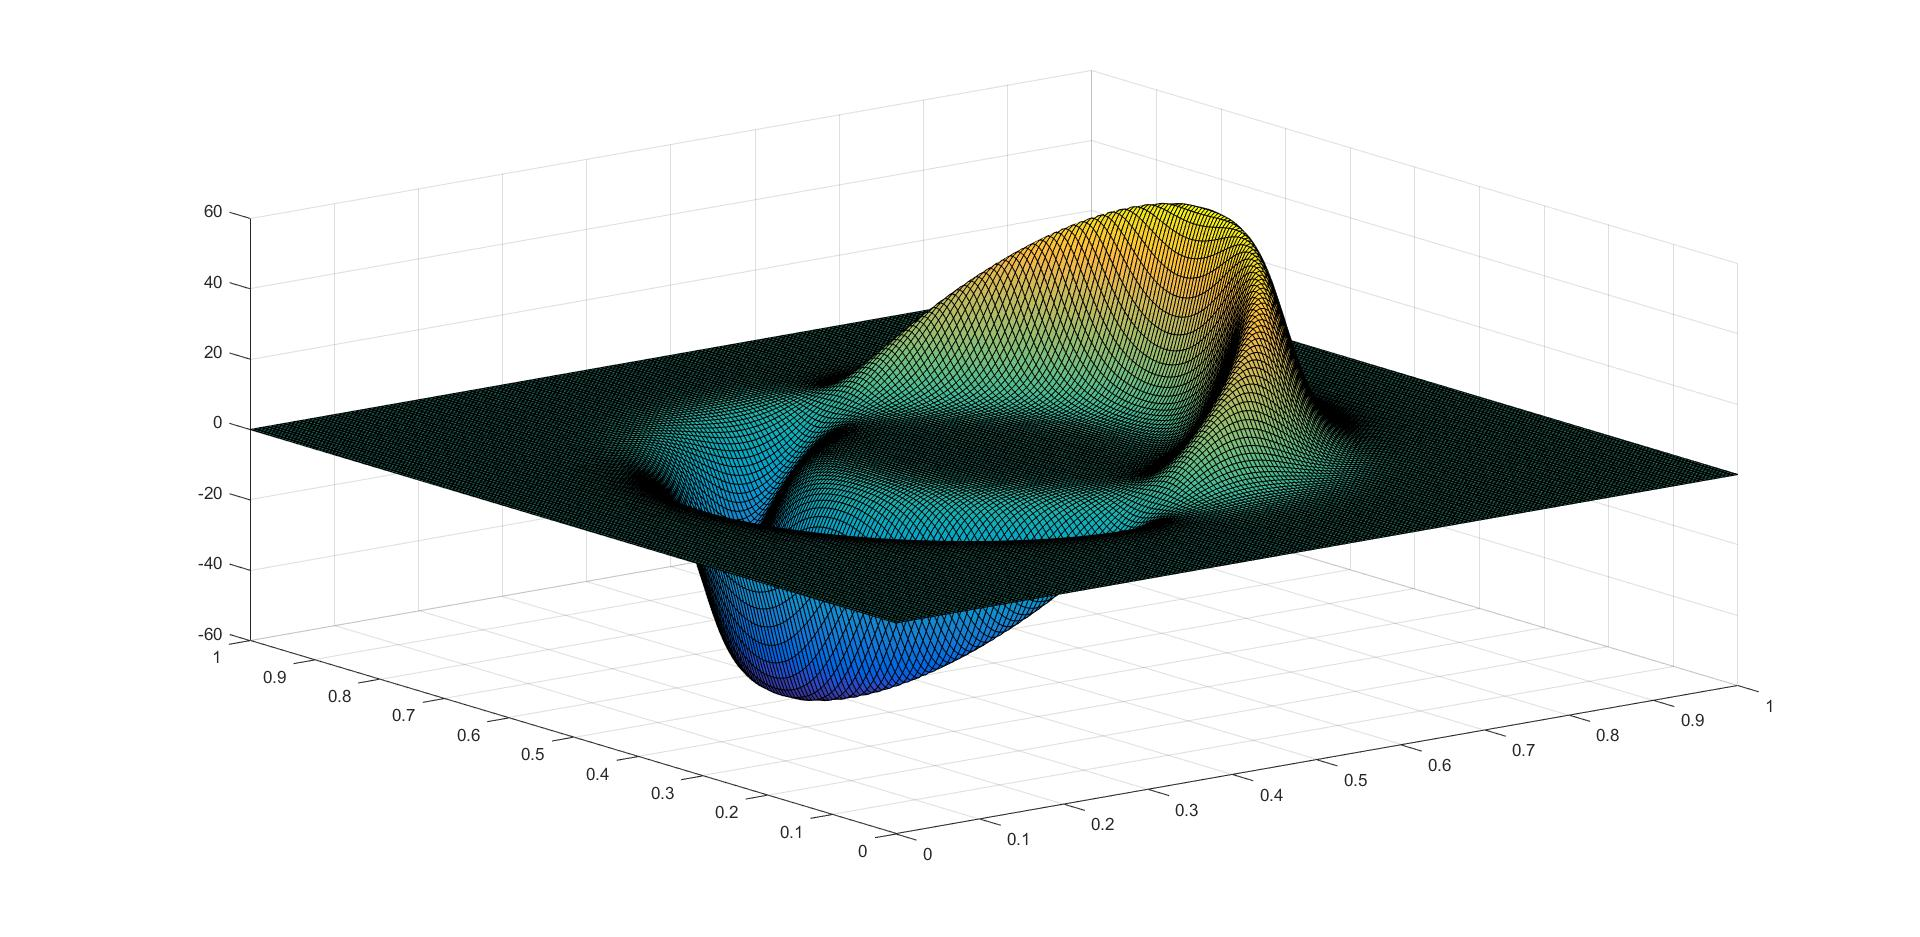
\includegraphics[width=\textwidth]{F3D.jpg}
            \caption{$F$的3维图片}\label{1.a}
        \end{subfigure}
        \begin{subfigure}[t]{0.49\textwidth}
            \centering
            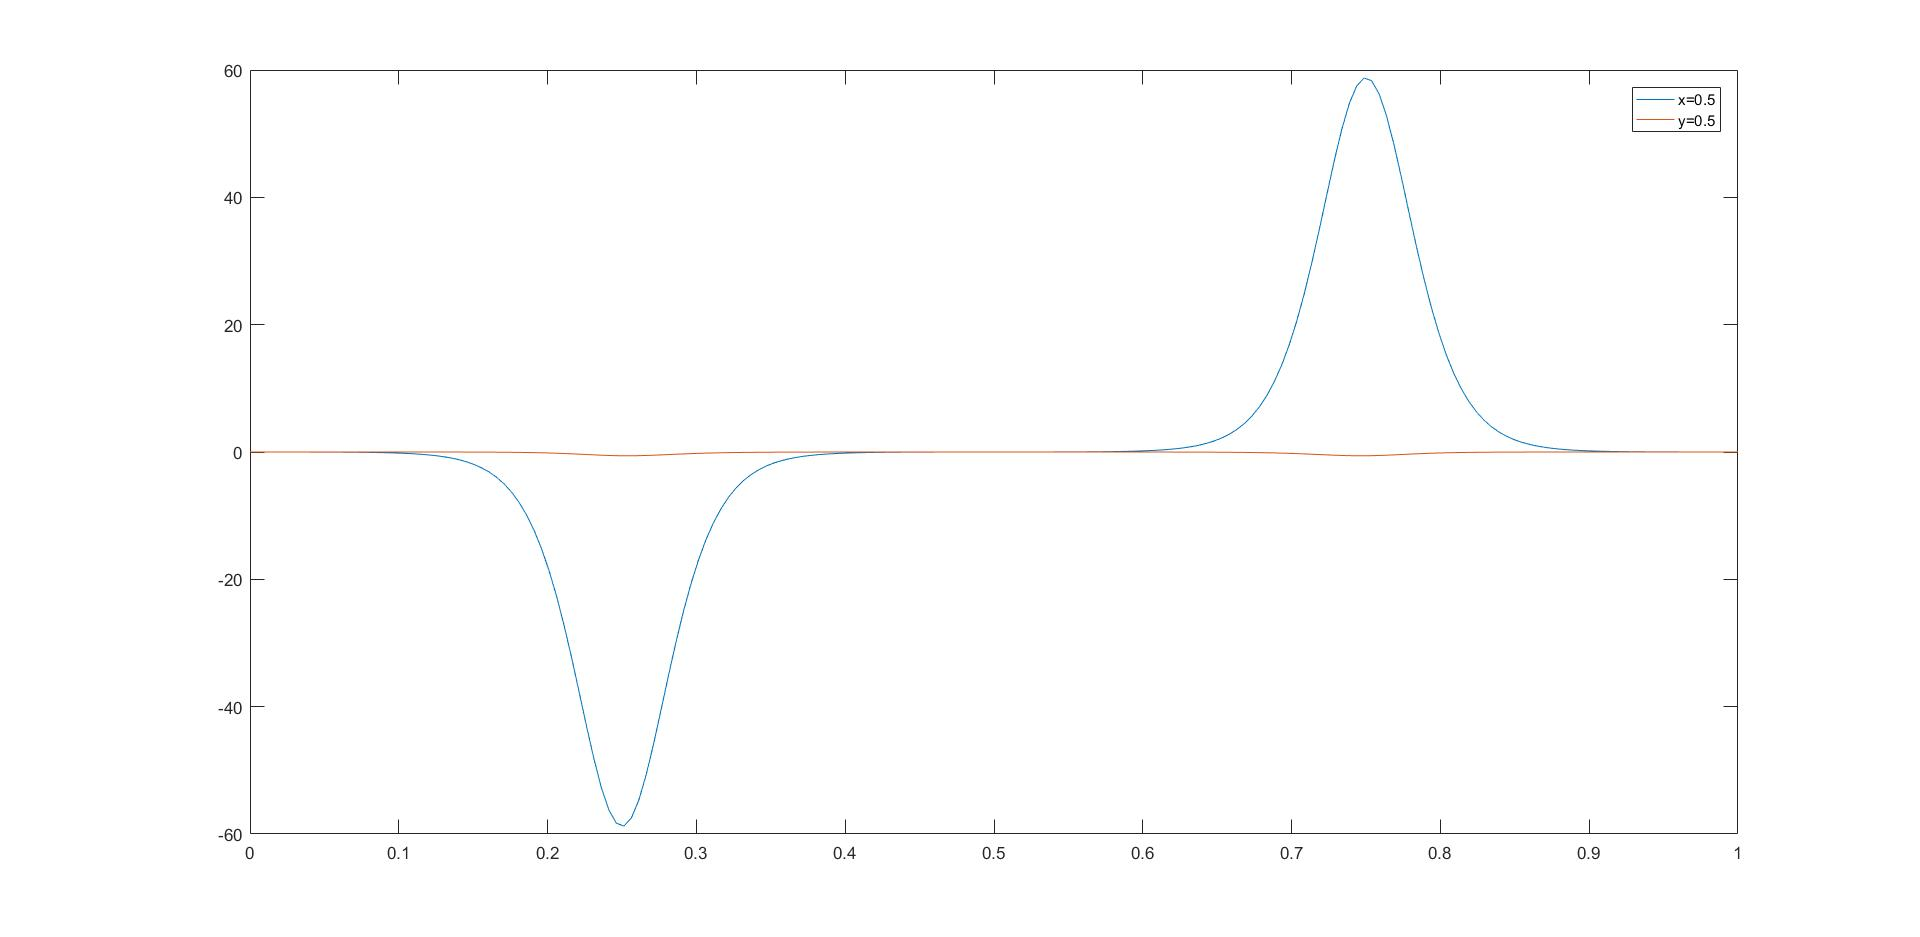
\includegraphics[width=\textwidth]{F2D.jpg}
            \caption{$F$在$x=0.5$$(y=0.5)$的投影}\label{1.b}
        \end{subfigure}
        \caption{$F$的图像}
    \end{figure}
    }
    \par{图2是力在给定的数值下的图像,图2.a为力的三维图像,图2.b为$F$在
    $x=0.5$$(y=0.5)$的投影。可以发现力的最大值为58.8,最小值为-58.8,负值
    出现的位置为圆形颗粒的上下边界附近,左右边界没有负值。从图像上来看
    整个系统并不是完全对称的,所以力在上下边界和左右边界有所不同也很正常。}
    \par{\textbf{REMARK:}对于库埃特流,其是具有不稳定库埃特流的精确解,其
    形式如下:
    $$
    u=U_0y/H-\frac{2U_0}{\pi}\sum_{n=1}^{\infty}\frac{1}{n}e^{-n^2\pi^2\nu t/H^2}\sin[{n\pi(1-\frac{y}{H})]}
    $$
    针对本文模拟的数值实力,我们验证就算是带入截断的不稳定库埃特流的精确解的情况下,力
    的表达式也不会发生改变。首先需要利用NS方程:
    $$
    \rho[\frac{\partial u}{\partial t}+(u \cdot \nabla)u] = -\nabla p + (\nabla u)
    \nabla \eta + \eta \triangle u
    $$
    由于模拟选取的密度密度都假设为$\rho=1$,所以有$\eta=\nu$。将截断的不稳定库埃特流
    的精确解表达式代入NS方程,我们可以计算发现$\frac{\partial u}{\partial t}=
    \eta \triangle u$。}
    \par{最后我们验证对流项为0,即$(u \cdot \nabla)u=0$。$u$的分量表达式为:
    $$
     u=\left(
    \begin{array}{cc}
        u_x(y) \\
        u_y=0
    \end{array}
    \right)
    $$
    利用$u$的分量表达式,可以清晰的看见$u \cdot \nabla = 0$。于是NS方程即被化简为
    $$
    0 = -\nabla p + (\nabla u)\nabla \eta
    $$可见此数值算例中力的表达式在截断的不稳定库埃特流也是一样的。}
\end{document}